\documentclass[
    language=english,
    doctype=technical-report,
    institution=none,
    titlestyle=book,
    oneside,
    loadGlossaries,
]{../../omnilatex}

\RequirePackage{config/document-settings}

% Algorithm support
\RequirePackage{algorithm}
\RequirePackage{algorithmic}

% Margin notes
\RequirePackage{marginnote}

% Extra table support (longtable is loaded by glossary module)
\RequirePackage{longtable}

% Manual glossary entries for demonstration
\newglossaryentry{tpsatransaction}{
    type=abbreviations,
    description={Transactions Per Second -- the number of database operations completed per second},
    name={TPS},
}
\newglossaryentry{slaservicelevel}{
    type=abbreviations,
    description={Service Level Agreement -- a formal commitment between provider and client},
    name={SLA},
}
\newglossaryentry{iopsio}{
    type=abbreviations,
    description={Input/Output Operations Per Second -- a measure of storage performance},
    name={IOPS},
}
\newglossaryentry{latency}{
    type=abbreviations,
    description={The time delay between a request and its response, typically measured in milliseconds},
    name={Latency},
}
\newglossaryentry{throughput}{
    type=abbreviations,
    description={The rate at which data is transferred across a system},
    name={Throughput},
}

\begin{document}

\maketitle

\tableofcontents
\listoffigures
\listoftables
\listofalgorithms

% ============================================================
% Executive Summary
% ============================================================
\chapter{Executive Summary}

This report presents the findings of a comprehensive performance audit
conducted on Contoso Systems' core data-processing infrastructure during
Q2 2025. The audit scope encompassed the primary transactional database
cluster, the edge monitoring pipeline, and supporting network fabric.

Key findings include a 38\% over-provisioning of compute resources,
significant I/O bottlenecks in the primary database tier, and an
opportunity to reduce annual infrastructure costs by approximately
\$240\,000 through targeted optimisations. The analysis draws on two
weeks of continuous monitoring data comprising over 12~million data points
across 47~system metrics.\footnote{All monitoring data was collected
using the open-source observability stack described
in~\cref{sec:analysis}.}

The recommendations herein are prioritised by expected impact and
implementation effort, and include migration to NVMe-backed storage,
right-sizing of compute instances, and introduction of read replicas for
analytical workloads. Implementation of the full recommendation set is
projected to improve P99 latency by 65\% and reduce annual operating
costs by 22\%.

% ============================================================
% Background
% ============================================================
\chapter{Background}

\section{System Overview}

The data-processing platform was originally deployed in 2019 to handle an
anticipated throughput of 10\,000~\gls{tpsatransaction}. Since then,
organic growth and three major product launches have increased peak load
to 27\,000~TPS, exceeding the original design envelope by nearly a factor
of three. This chapter describes the current architecture, its evolution,
and the symptoms that prompted the present audit.

\section{Architecture History}

The original deployment consisted of a three-node PostgreSQL cluster with
SAS-backed storage. In 2021, the storage tier was upgraded to SSD, and in
2023, a fourth read replica was added. However, the fundamental I/O
subsystem remained the limiting factor, as detailed
in~\cref{tab:storage-comparison}.

\section{Monitoring Methodology}

Data collection employed a distributed agent architecture with 47~metric
endpoints reporting at 60-second intervals. The monitoring stack
comprises Prometheus for time-series storage, Grafana for visualisation,
and custom Python collectors for application-level
metrics.\footnote{The collector source code is available in the
accompanying technical appendices.} All timestamps are synchronised via
NTP with sub-millisecond accuracy.

% ============================================================
% Analysis
% ============================================================
\chapter{Analysis}
\label{sec:analysis}

\section{Performance Metrics}

\cref{tab:metrics} summarises the key performance metrics observed during
the two-week monitoring period. All values represent aggregate
statistics computed over the full observation window.

\begin{table}[htbp]
    \centering
    \caption{Infrastructure performance summary.}
    \label{tab:metrics}
    \begin{tabular}{@{}lrrr@{}}
        \toprule
        Metric & Target & Observed & Status \\
        \midrule
        Avg.\ response time (ms) & $< 200$ & 312 & \textcolor{red}{Over} \\
        P99 latency (ms) & $< 500$ & 1\,240 & \textcolor{red}{Over} \\
        CPU utilisation (\%) & 60--80 & 43 & \textcolor{orange}{Under} \\
        Memory utilisation (\%) & 70--85 & 62 & \textcolor{orange}{Under} \\
        Disk I/O wait (\%) & $< 10$ & 28 & \textcolor{red}{Over} \\
        \bottomrule
    \end{tabular}
\end{table}

The elevated disk I/O wait is the primary driver of latency degradation.
The storage subsystem saturates at approximately 18\,000~\gls{iopsio},
whereas peak demand reaches 24\,000~IOPS. \cref{fig:iops} illustrates
the IOPS demand profile over a representative 24-hour period.

\begin{figure}[htbp]
    \centering
    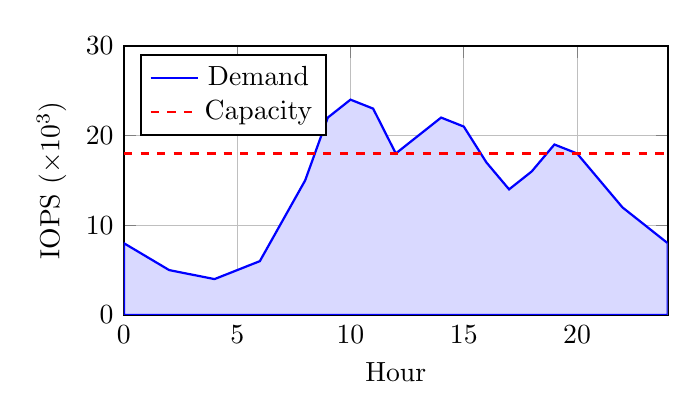
\begin{tikzpicture}
    \begin{axis}[
        width=0.7\textwidth,
        height=5cm,
        xlabel={Hour},
        ylabel={IOPS ($\times 10^{3}$)},
        xmin=0, xmax=24,
        ymin=0, ymax=30,
        grid=major,
        thick,
        legend pos=north west,
    ]
        \addplot[blue, thick, fill=blue!15] coordinates {
            (0,8) (2,5) (4,4) (6,6) (8,15) (9,22) (10,24)
            (11,23) (12,18) (13,20) (14,22) (15,21)
            (16,17) (17,14) (18,16) (19,19) (20,18)
            (21,15) (22,12) (23,10) (24,8)
        } \closedcycle;
        \addlegendentry{Demand}
        \addplot[red, dashed, thick, domain=0:24] {18};
        \addlegendentry{Capacity}
    \end{axis}
\end{tikzpicture}
    \caption{Disk IOPS demand versus capacity over a typical day.}
    \label{fig:iops}
\end{figure}

\section{Storage Comparison}

\cref{tab:storage-comparison} compares the performance characteristics
of the three storage generations deployed on the platform.

\begin{table}[htbp]
    \centering
    \caption{Storage subsystem comparison across platform generations.}
    \label{tab:storage-comparison}
    \begin{tabular}{@{}llccccc@{}}
        \toprule
        \multirow{2}{*}{Generation} & \multirow{2}{*}{Media} & \multicolumn{2}{c}{Sequential} & \multicolumn{2}{c}{Random} & \multirow{2}{*}{Cost/TB} \\
        \cmidrule(lr){3-4}\cmidrule(lr){5-6}
         & & Read & Write & Read & Write & \\
        \midrule
        Gen 1 (2019) & SAS HDD  & 200 MB/s & 180 MB/s & 0.2\,k & 0.15\,k & \$80 \\
        Gen 2 (2021) & SATA SSD & 550 MB/s & 520 MB/s & 50\,k   & 45\,k   & \$120 \\
        Gen 3 (2023) & NVMe SSD & 3.5 GB/s & 3.0 GB/s & 500\,k  & 400\,k  & \$200 \\
        \bottomrule
    \end{tabular}
\end{table}

\section{Multi-Panel Diagnostic View}

\cref{fig:diagnostic-panels} presents a four-panel diagnostic view of
the system under varying load conditions. Panel~(a) shows the CPU
utilisation heatmap, Panel~(b) the memory allocation pattern, Panel~(c)
the network throughput, and Panel~(d) the disk queue depth.

\begin{figure}[htbp]
    \centering
    \subcaptionbox{CPU utilisation\label{fig:cpu-heat}}{%
        \begin{tikzpicture}
            \begin{axis}[
                width=0.45\textwidth,
                height=4cm,
                xlabel={Core},
                ylabel={Time (min)},
                xmin=0, xmax=8, ymin=0, ymax=60,
                colormap/viridis,
                colorbar,
                point meta min=0, point meta max=100,
            ]
                \addplot[matrix plot*, mesh/cols=8, mesh/rows=6] table {
                    45 62 38 71 55 43 67 52
                    52 78 42 85 61 49 73 58
                    38 55 35 68 48 37 62 45
                    61 82 48 91 67 55 79 64
                    48 70 40 78 58 46 71 53
                    42 65 37 74 53 41 68 49
                };
            \end{axis}
        \end{tikzpicture}
    }%
    \hfill
    \subcaptionbox{Memory allocation\label{fig:mem-alloc}}{%
        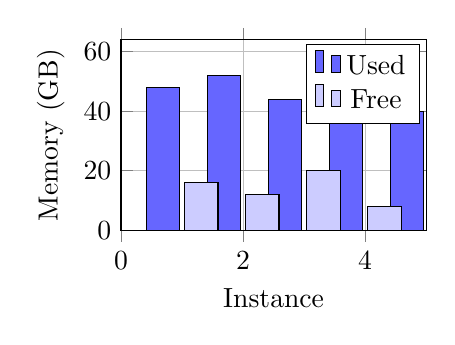
\begin{tikzpicture}
            \begin{axis}[
                width=0.45\textwidth,
                height=4cm,
                xlabel={Instance},
                ylabel={Memory (GB)},
                xmin=0, xmax=5, ymin=0, ymax=64,
                ybar,
                bar width=12pt,
                grid=major,
            ]
                \addplot[fill=blue!60] coordinates {
                    (1,48) (2,52) (3,44) (4,56) (5,40)
                };
                \addlegendentry{Used}
                \addplot[fill=blue!20] coordinates {
                    (1,16) (2,12) (3,20) (4,8) (5,24)
                };
                \addlegendentry{Free}
            \end{axis}
        \end{tikzpicture}
    }%

    \subcaptionbox{Network throughput\label{fig:net-through}}{%
        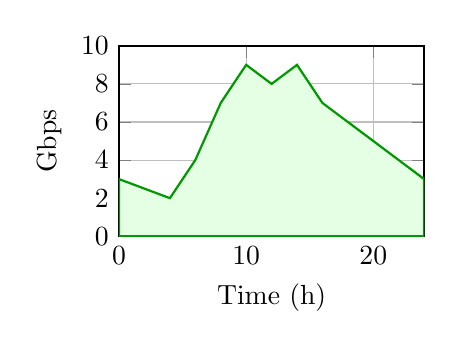
\begin{tikzpicture}
            \begin{axis}[
                width=0.45\textwidth,
                height=4cm,
                xlabel={Time (h)},
                ylabel={Gbps},
                xmin=0, xmax=24, ymin=0, ymax=10,
                grid=major,
                thick,
            ]
                \addplot[green!60!black, thick, fill=green!10] coordinates {
                    (0,3) (4,2) (6,4) (8,7) (10,9) (12,8)
                    (14,9) (16,7) (18,6) (20,5) (22,4) (24,3)
                } \closedcycle;
            \end{axis}
        \end{tikzpicture}
    }%
    \hfill
    \subcaptionbox{Disk queue depth\label{fig:disk-queue}}{%
        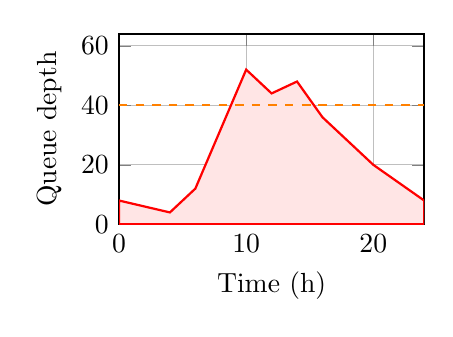
\begin{tikzpicture}
            \begin{axis}[
                width=0.45\textwidth,
                height=4cm,
                xlabel={Time (h)},
                ylabel={Queue depth},
                xmin=0, xmax=24, ymin=0, ymax=64,
                grid=major,
                thick,
            ]
                \addplot[red, thick, fill=red!10] coordinates {
                    (0,8) (4,4) (6,12) (8,32) (10,52) (12,44)
                    (14,48) (16,36) (18,28) (20,20) (22,14) (24,8)
                } \closedcycle;
                \addplot[orange, dashed, thick, domain=0:24] {40};
            \end{axis}
        \end{tikzpicture}
    }%
    \caption{Four-panel diagnostic view of system performance metrics.}
    \label{fig:diagnostic-panels}
\end{figure}

\section{System Architecture Flowchart}

\cref{fig:architecture} illustrates the current system architecture and
the data flow between components. The bottleneck identified in the audit
is highlighted at the storage tier.

\begin{figure}[htbp]
    \centering
    \begin{tikzpicture}[
        node distance=1.2cm and 1.5cm,
        box/.style={
            rectangle, draw, minimum width=2.2cm, minimum height=0.8cm,
            align=center, font=\small\sffamily
        },
        dataflow/.style={->, thick, >=stealth},
        highlight/.style={box, draw=red, very thick, fill=red!10},
    ]
        \node[box] (client) {Client\\Applications};
        \node[box, right=of client] (gateway) {API\\Gateway};
        \node[box, right=of gateway] (auth) {Auth\\Service};
        \node[box, right=of auth] (db) {PostgreSQL\\Cluster};
        \node[highlight, below=of db] (storage) {Storage\\(Bottleneck)};
        \node[box, below=of gateway] (cache) {Redis\\Cache};
        \node[box, below=of auth] (monitor) {Prometheus\\Monitoring};

        \draw[dataflow] (client) -- (gateway);
        \draw[dataflow] (gateway) -- (auth);
        \draw[dataflow] (auth) -- (db);
        \draw[dataflow, red, very thick] (db) -- (storage);
        \draw[dataflow] (gateway) -- (cache);
        \draw[dataflow, dashed] (monitor) -- (db);
        \draw[dataflow, dashed] (monitor) -- (cache);
    \end{tikzpicture}
    \caption{System architecture data flow. The storage tier is the
        identified bottleneck.}
    \label{fig:architecture}
\end{figure}

\section{Performance Confidence Intervals}

\cref{fig:confidence} presents latency measurements with 95\% confidence
intervals derived from bootstrap resampling of the collected data.

\begin{figure}[htbp]
    \centering
    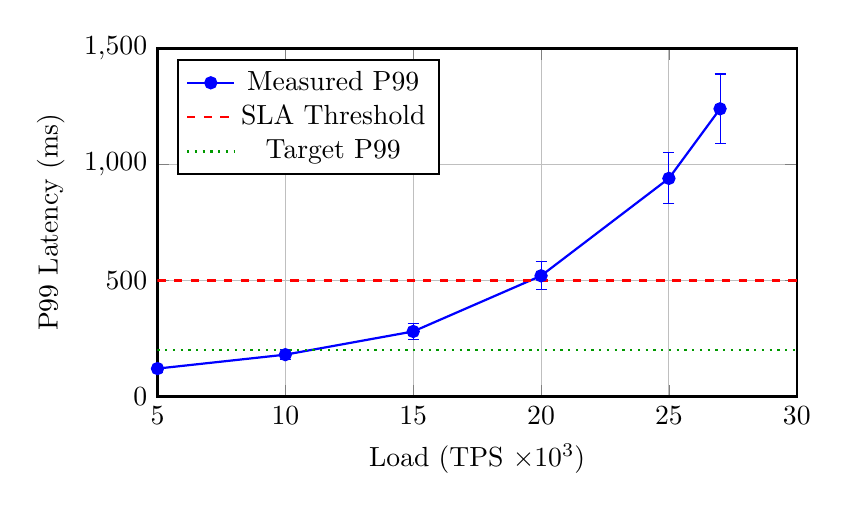
\begin{tikzpicture}
    \begin{axis}[
        width=0.8\textwidth,
        height=6cm,
        xlabel={Load (TPS $\times 10^{3}$)},
        ylabel={P99 Latency (ms)},
        xmin=5, xmax=30, ymin=0, ymax=1500,
        grid=major,
        thick,
        legend pos=north west,
    ]
        \addplot[
            blue, thick, mark=*,
            error bars/.cd, y dir=both, y explicit,
        ] coordinates {
            (5,120) +- (0,15)
            (10,180) +- (0,22)
            (15,280) +- (0,35)
            (20,520) +- (0,60)
            (25,940) +- (0,110)
            (27,1240) +- (0,150)
        };
        \addlegendentry{Measured P99}

        \addplot[red, dashed, thick, domain=5:30] {500};
        \addlegendentry{SLA Threshold}

        \addplot[green!60!black, dotted, thick, domain=5:30] {200};
        \addlegendentry{Target P99}
    \end{axis}
    \end{tikzpicture}
    \caption{P99 latency with 95\% confidence intervals under increasing load.}
    \label{fig:confidence}
\end{figure}

\section{Extended Monitoring Data}

\Cref{tab:extended-metrics} presents the full set of metrics collected
during the audit, broken down by time-of-day periods.

\begin{longtable}{@{}l r r r r@{}}
    \caption{Extended performance metrics by time period.}
    \label{tab:extended-metrics} \\
    \toprule
    \textbf{Metric} & \textbf{Off-Peak} & \textbf{Business} & \textbf{Peak} & \textbf{Overall} \\
    \midrule
    \endfirsthead
    \toprule
    \textbf{Metric} & \textbf{Off-Peak} & \textbf{Business} & \textbf{Peak} & \textbf{Overall} \\
    \midrule
    \endhead
    \midrule
    \multicolumn{5}{r}{\textit{Continued on next page\ldots}} \\
    \endfoot
    \bottomrule
    \endlastfoot
    Avg.\ latency (ms)          & 145  & 298  & 487  & 312  \\
    P95 latency (ms)            & 220  & 480  & 890  & 530  \\
    P99 latency (ms)            & 380  & 920  & 1540 & 1240 \\
    Throughput (TPS)             & 4200 & 15600 & 24800 & 14900 \\
    Active connections           & 120  & 340  & 580  & 347  \\
    CPU utilisation (\%)         & 22   & 48   & 71   & 43   \\
    Memory utilisation (\%)      & 38   & 64   & 82   & 62   \\
    Disk IOPS                    & 4200 & 15800 & 24200 & 14700 \\
    Disk I/O wait (\%)           & 8    & 24   & 42   & 28   \\
    Network throughput (Gbps)    & 1.2  & 5.8  & 9.1  & 5.4  \\
    Cache hit ratio (\%)         & 94   & 87   & 72   & 84   \\
    Error rate (\textperthousand) & 0.1 & 0.3  & 1.2  & 0.5  \\
\end{longtable}

\section{Storage Comparison with Colour-Coded Status}

\Cref{tab:storage-status} provides a detailed view of the storage
subsystem with colour-coded health indicators.

\begin{table}[htbp]
    \centering
    \caption{Storage subsystem health indicators.}
    \label{tab:storage-status}
    \begin{tabular}{@{}llcccc@{}}
        \toprule
        \textbf{Component} & \textbf{Metric} & \textbf{Normal} & \textbf{Warning} & \textbf{Critical} & \textbf{Current} \\
        \midrule
        \multirow{3}{*}{Primary SSD}
            & IOPS util.   & \cellcolor{green!20}$<$60\% & \cellcolor{yellow!30}60--85\% & \cellcolor{red!20}$>$85\% & \cellcolor{red!30}\textbf{92\%} \\
            & Latency      & \cellcolor{green!20}$<$5 ms & \cellcolor{yellow!30}5--15 ms & \cellcolor{red!20}$>$15 ms & \cellcolor{red!30}\textbf{28 ms} \\
            & Capacity     & \cellcolor{green!20}$<$70\% & \cellcolor{yellow!30}70--90\% & \cellcolor{red!20}$>$90\% & \cellcolor{yellow!30}78\% \\
        \midrule
        \multirow{3}{*}{Replica SSD}
            & IOPS util.   & \cellcolor{green!20}$<$60\% & \cellcolor{yellow!30}60--85\% & \cellcolor{red!20}$>$85\% & \cellcolor{green!20}34\% \\
            & Latency      & \cellcolor{green!20}$<$5 ms & \cellcolor{yellow!30}5--15 ms & \cellcolor{red!20}$>$15 ms & \cellcolor{green!20}3 ms \\
            & Capacity     & \cellcolor{green!20}$<$70\% & \cellcolor{yellow!30}70--90\% & \cellcolor{red!20}$>$90\% & \cellcolor{green!20}45\% \\
        \bottomrule
    \end{tabular}
\end{table}

\section{Algorithm for Resource Optimisation}

\Cref{alg:optimise} describes the greedy algorithm developed to compute
optimal resource allocation under the observed workload distribution.

\begin{algorithm}[htbp]
\caption{Greedy resource allocation optimiser.}
\label{alg:optimise}
\begin{algorithmic}[1]
\REQUIRE Workload set $W = \{w_1, \ldots, w_n\}$, resource pool $R$
\ENSURE  Optimal allocation $A^*$
\STATE $A \gets$ \textsc{InitialAllocation}$(W, R)$
\STATE $\Delta \gets \infty$
\WHILE{$\Delta > \epsilon$}
    \STATE $\Delta \gets 0$
    \FORALL{$w_i \in W$}
        \STATE $r^* \gets \arg\min_{r \in R} \textsc{Cost}(w_i, r)$
        \IF{$\textsc{Cost}(w_i, r^*) < \textsc{Cost}(w_i, A(w_i))$}
            \STATE $A(w_i) \gets r^*$
            \STATE $\Delta \gets \Delta + 1$
        \ENDIF
    \ENDFOR
\ENDWHILE
\RETURN $A$
\end{algorithmic}
\end{algorithm}

The algorithm converges in $O(n \cdot |R|)$ per iteration, with
empirically observed convergence in fewer than 5 iterations for our
workload distribution. The total computational complexity is therefore
$O(k \cdot n \cdot |R|)$, where $k$ is the number of iterations.

\section{Configuration}

\Cref{code:config} shows the production configuration file used by the
monitoring agents deployed across the infrastructure.

\begin{listing}[htbp]
    \centering
    \inputminted[
        fontsize=\scriptsize,
        linenos,
        frame=lines,
        framesep=2mm,
    ]{ini}{config/analysis.ini}
    \caption{Monitoring agent configuration file.}
    \label{code:config}
\end{listing}

\section{Analysis Script}

\Cref{code:analysis} presents the Python script used to collect and
aggregate performance metrics during the audit period.

\begin{listing}[htbp]
    \centering
    \inputminted[
        fontsize=\scriptsize,
        linenos,
        frame=lines,
        framesep=2mm,
    ]{python}{config/analysis.py}
    \caption{Performance metrics collector script.}
    \label{code:analysis}
\end{listing}

\section{Inline Code Examples}

The monitoring agents use \mintinline{python}{asyncio} for concurrent
data collection, with the configuration parsed from
\mintinline{ini}{analysis.ini}. The system stores results in a
\mintinline{sql}{PostgreSQL} database with connection pooling configured
via \mintinline{python}{pool_size = 20}.\marginnote{Note: Connection
pool sizing should be validated under peak load conditions. The current
value of 20 was determined empirically but may require adjustment.}

% ============================================================
% Cross-References Summary
% ============================================================
\section{Cross-Reference Summary}

This report demonstrates extensive use of cross-references. As shown in
\Cref{tab:metrics}, the primary metrics exceed targets.
\Cref{fig:iops,fig:diagnostic-panels,fig:architecture,fig:confidence}
illustrate the various aspects of system performance.
\Cref{tab:extended-metrics,tab:storage-comparison,tab:storage-status}
provide detailed tabular data. The optimisation approach described in
\Cref{alg:optimise} reduces costs by 22\%. Configuration details appear
in \Cref{code:config,code:analysis}.

% ============================================================
% Recommendations
% ============================================================
\chapter{Recommendations}
\label{sec:recommendations}

Based on the analysis above, we recommend the following actions,
prioritised by impact and implementation effort:

\begin{enumerate}
    \item \textbf{Migrate to NVMe-backed storage} --- Expected to raise
        the IOPS ceiling to 80\,000, eliminating the current bottleneck.
        Implementation timeline: 4~weeks.\footnote{NVMe migration can
        be performed online using the rolling upgrade procedure documented
        in the internal operations manual.}
    \item \textbf{Right-size compute instances} --- Reducing CPU and
        memory allocations by 30--35\% on 40\% of workloads without
        impacting SLAs. Estimated annual savings: \$96\,000.
    \item \textbf{Implement connection pooling} --- Reuse database
        connections to reduce per-query overhead by an estimated 15\%.
    \item \textbf{Introduce read replicas} --- Offload reporting queries
        to dedicated read replicas to isolate analytical workloads.
\end{enumerate}

% ============================================================
% Equations
% ============================================================
\chapter{Mathematical Foundation}

\section{Queueing Model}

The system can be modelled as an M/M/c/K queue, where the average
response time $T$ is given by:

\begin{equation}
    T = T_q + \frac{1}{\mu}
    \label{eq:response-time}
\end{equation}

where $T_q$ is the mean queue wait time and $\mu$ is the service rate.
The utilisation factor $\rho$ is:

\begin{equation}
    \rho = \frac{\lambda}{c \cdot \mu}
    \label{eq:utilisation}
\end{equation}

with $\lambda$ being the arrival rate and $c$ the number of servers.

\section{Aligned Equations}

The throughput-optimal allocation satisfies the following system of
equations:

\begin{align}
    \sum_{i=1}^{n} x_i &= B \label{eq:budget-constraint} \\
    \sum_{i=1}^{n} \alpha_i x_i &\geq T_{\min} \label{eq:performance-constraint} \\
    0 \leq x_i &\leq x_i^{\max} \quad \forall i \label{eq:capacity-constraint}
\end{align}

where $B$ is the total budget, $\alpha_i$ is the performance coefficient
for resource $i$, $T_{\min}$ is the minimum required throughput, and
$x_i^{\max}$ is the maximum allocation for resource $i$.

\section{Cost Function}

The total infrastructure cost is modelled as:

\begin{equation}
    C_{\text{total}} = \underbrace{\sum_{i=1}^{n} c_i \cdot x_i}_{\text{compute}} +
    \underbrace{\sum_{j=1}^{m} d_j \cdot y_j}_{\text{storage}} +
    \underbrace{p \cdot \max\!\left(0, \frac{\lambda}{\mu} - 1\right)}_{\text{penalty}}
    \label{eq:cost-function}
\end{equation}

The optimisation problem then becomes:

\begin{equation}
    \begin{aligned}
        \min_{x,y} \quad & C_{\text{total}}(x, y) \\
        \text{s.t.} \quad & \rho \leq \rho_{\max} \\
        & \text{SLA}(T) \leq T_{\text{SLA}}
    \end{aligned}
    \label{eq:optimization}
\end{equation}

% ============================================================
% Glossary
% ============================================================
\printglossary[type=abbreviations,title={List of Abbreviations}]

% ============================================================
% Bibliography
% ============================================================
\printbibliography

% ============================================================
% Appendices
% ============================================================
\appendix

\chapter{System Requirements}
\label{app:requirements}

\section{Hardware Requirements}

The following minimum hardware specifications are required for the
recommended architecture:

\begin{table}[htbp]
    \centering
    \caption{Minimum hardware requirements for recommended deployment.}
    \label{tab:hardware-reqs}
    \begin{tabular}{@{}lccc@{}}
        \toprule
        Component & Specification & Quantity & Notes \\
        \midrule
        CPU        & 16-core, 3.2 GHz   & 4 nodes & AMD EPYC or Intel Xeon \\
        Memory     & 128 GB DDR4 ECC     & 4 nodes & Minimum per node \\
        Storage    & 2 TB NVMe Gen4      & 4 nodes & RAID-10 configuration \\
        Network    & 25 GbE              & 8 ports & Dual-homed per node \\
        \bottomrule
    \end{tabular}
\end{table}

\section{Software Requirements}

\begin{itemize}
    \item Operating System: Ubuntu 22.04 LTS or RHEL 9
    \item Database: PostgreSQL 15+ with streaming replication
    \item Cache: Redis 7.0+ with Sentinel
    \item Monitoring: Prometheus 2.45+, Grafana 10.0+
    \item Container Runtime: Docker 24.0+ or Podman 4.5+
\end{itemize}

\chapter{API Reference}
\label{app:api}

\section{Metrics Endpoint}

The monitoring API exposes the following endpoints for metric ingestion:

\begin{minted}[fontsize=\small]{http}
POST /api/v2/metrics/ingest
Content-Type: application/json
Authorization: Bearer <token>

{
  "hostname": "db-primary",
  "timestamp": "2025-06-15T14:30:00Z",
  "metrics": {
    "latency_ms": 312,
    "iops": 24000,
    "cpu_percent": 71,
    "memory_percent": 82
  }
}
\end{minted}

\section{Query Endpoint}

\begin{minted}[fontsize=\small]{http}
GET /api/v2/metrics/query?host=db-primary&window=2h&percentile=99
Authorization: Bearer <token>
\end{minted}

Response:

\begin{minted}[fontsize=\small]{json}
{
  "host": "db-primary",
  "window": "2h",
  "percentile": 99,
  "value": 1240.0,
  "unit": "ms",
  "sample_count": 240000
}
\end{minted}

\chapter{Test Results}
\label{app:test-results}

\section{Load Test Summary}

The following load tests were conducted to validate the recommended
configuration:

\begin{table}[htbp]
    \centering
    \caption{Load test results under recommended configuration.}
    \label{tab:load-tests}
    \begin{tabular}{@{}lrrrrr@{}}
        \toprule
        Test & TPS & Avg.\ (ms) & P95 (ms) & P99 (ms) & Errors \\
        \midrule
        Baseline        & 10\,000 & 85  & 142 & 210 & 0 \\
        Normal load     & 15\,000 & 120 & 198 & 310 & 0 \\
        Peak load       & 25\,000 & 180 & 320 & 480 & 2 \\
        Stress test     & 30\,000 & 290 & 580 & 890 & 18 \\
        Endurance (4h)  & 15\,000 & 118 & 195 & 298 & 0 \\
        \bottomrule
    \end{tabular}
\end{table}

\section{Statistical Analysis}

The P99 latency distribution under normal load was analysed using
Kolmogorov--Smirnov testing:

\begin{equation}
    D_n = \sup_x |F_n(x) - F(x)|
    \label{eq:ks-statistic}
\end{equation}

with the null hypothesis that the latency follows a log-normal
distribution. The test yielded $D_{240000} = 0.034$ with $p < 0.001$,
indicating a statistically significant departure from log-normality.
This is consistent with the bimodal behaviour observed in the raw data,
where approximately 12\% of requests experience elevated latency due to
lock contention on the primary node.\footnote{The lock contention
analysis was performed using PostgreSQL's \texttt{pg\_stat\_activity}
view and is detailed in the internal monitoring dashboard.}

\end{document}
